\small

\begin{multicols}{2}
\section*{Impact}
Six years after the beginnings of the project, ObsPy is used by
seismologists all around the world. With \textbf{more than 500 downloads for
Debian/Ubuntu Linux alone}, we estimate -- including Mac, Windows and other
Linux/Unix users -- an \textbf{active user base of around 1000-2000 people}.

Since ObsPy's start by a \textbf{core developer team of 3-5 people} at LMU Munich, ObsPy
has evolved into a community effort with \textbf{contributions to the code base
by 40 individuals}. The \textbf{percentage of contributions from outside the core
developer team is constantly on the rise and is currently at around 40\%}.

The user mailing list currently has over \textbf{300 subscribers} and serves as a
place for discussions and asking for help from more experienced users.

The \textbf{impact of ObsPy and the appreciation within the seismological
community} finds expression in the \textbf{rapidly increasing number of scientific
citations, which stands at over 70 as of October 2014}.
%\begin{itemize}
%    \item Around 25 people contributed code so far
%    \item Estimated active user base of \textbf{more than 5000} people
%    \item Code hosted on Github $\Rightarrow$ Anyone can contribute
%    \item Mature and stable code base
%    \item Stable development process
%    \item Runs everywhere
%    \item Goal: Built enough momentum for ObsPy to be self-sustainable
%\end{itemize}
%
%\vspace{2ex}
%
\columnbreak
\begin{center}
    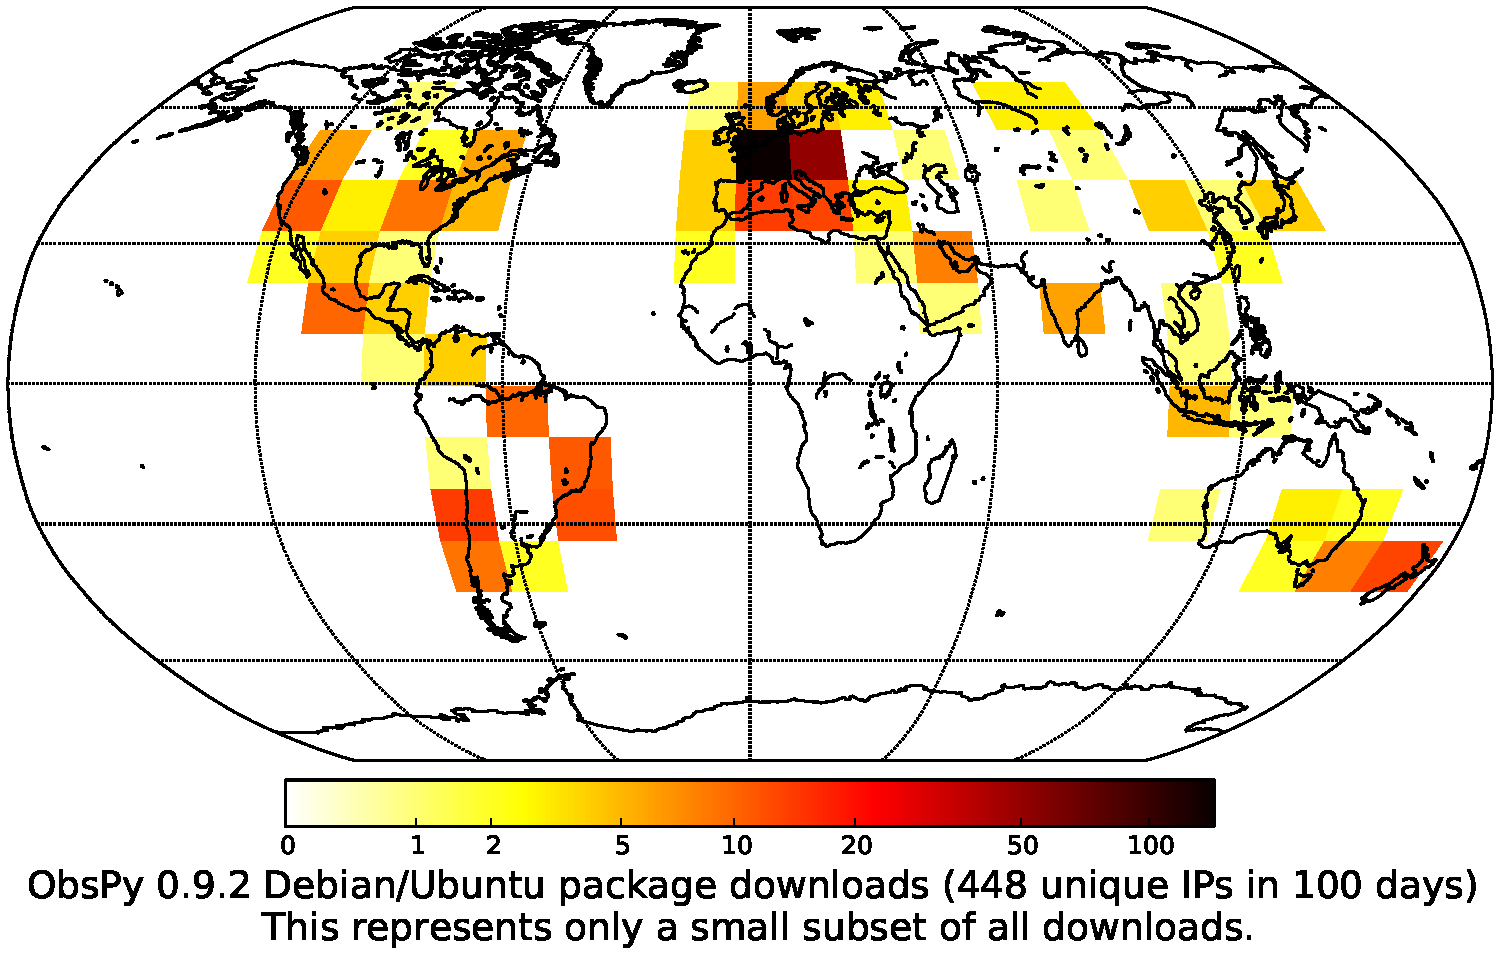
\includegraphics[width=0.8\columnwidth]{./images/obspy-deb.pdf} \\
\end{center}

\begin{center}
    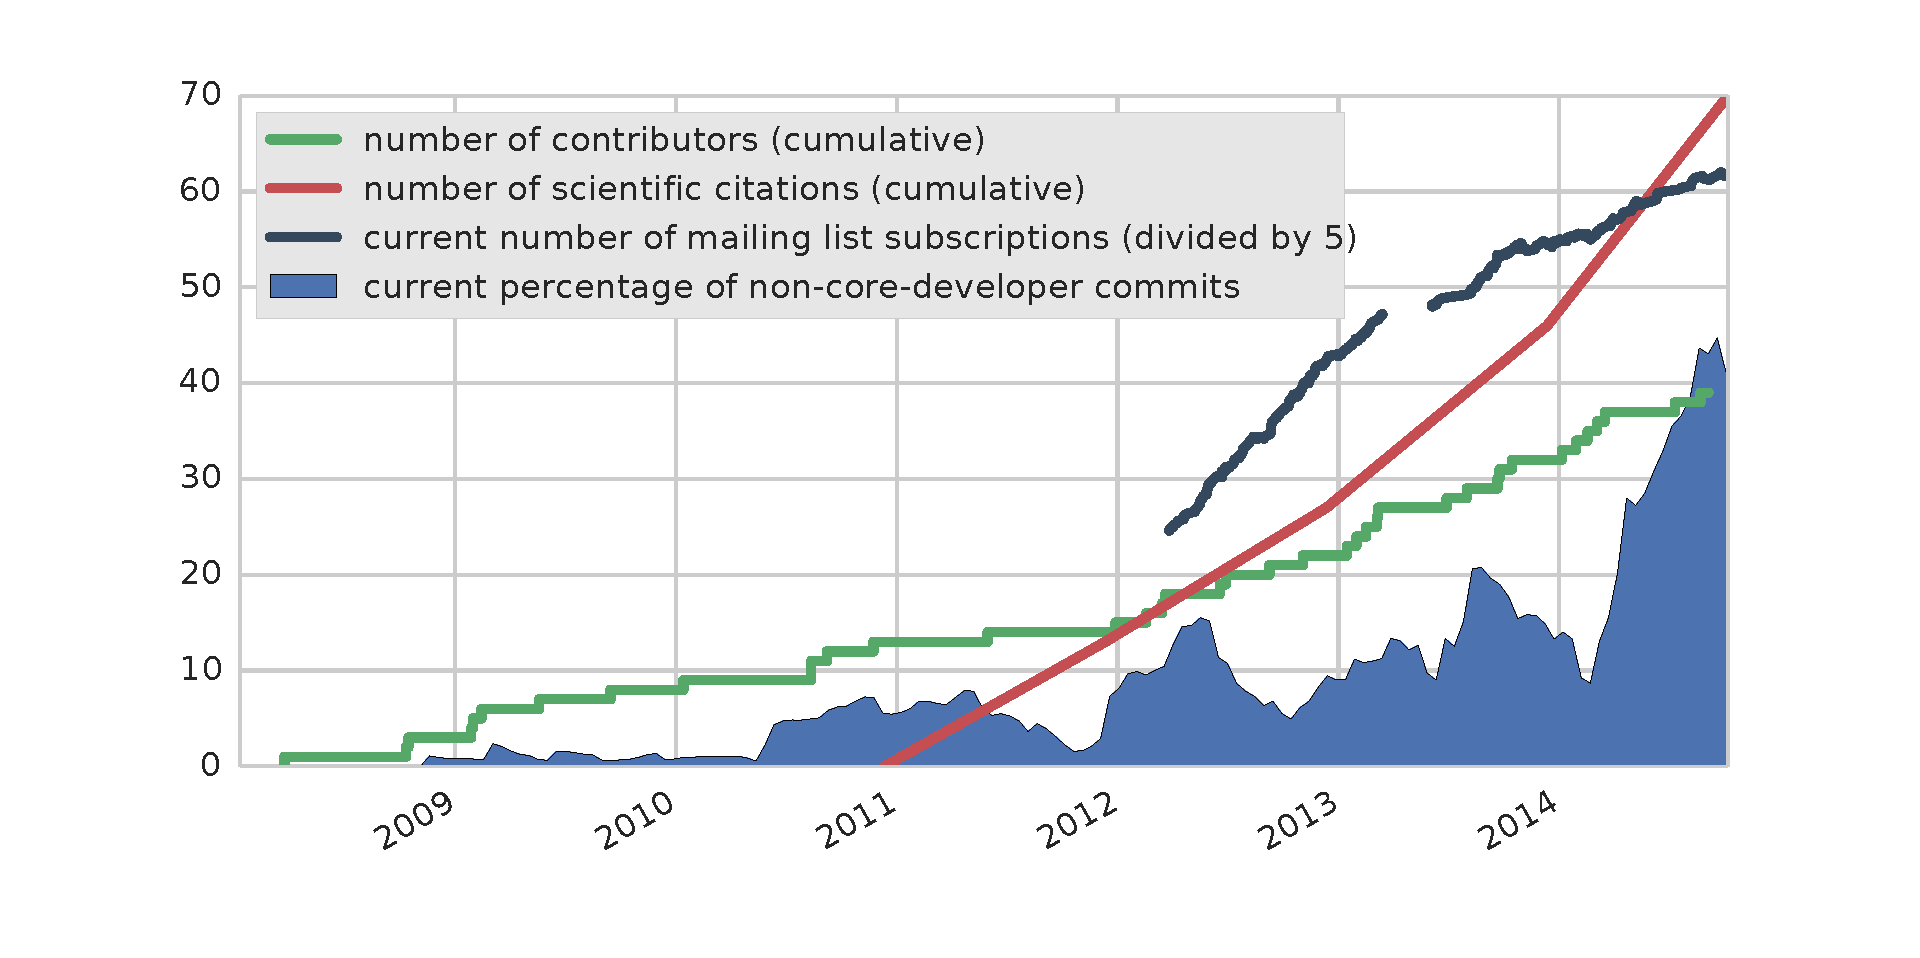
\includegraphics[width=1.0\columnwidth]{./images/all_stats.pdf} \\
\end{center}
\end{multicols}
